%-------------------------------------------------------------------------------
% yum_addsynth
%-------------------------------------------------------------------------------
%
% \file        yum_addsynth.tex
% \library     Documents
% \author      Chris Ahlstrom
% \date        2015-06-07
% \update      2015-07-04
% \version     $Revision$
% \license     $XPC_GPL_LICENSE$
%
%     Provides the ADDsynth section of yoshimi-user-manual.tex.
%
%-------------------------------------------------------------------------------

\section{ADDsynth}
\label{sec:addsynth}

   The \textsl{Yoshimi} ADDsynth (also spelled "ADsynth")
   dialog is a complex dialog for creating an
   instrument.  This is the most complex, most advanced and most
   sophisticated part of the synthesizer and allows one to edit the
   parameters that apply to all the voices of ADDsynth.

   ADDSynth, a primarily additive synthesis engine, is one of the three major
   synthesis engines available in ZynAddSubFX. The basic concept of this
   engine is the summation of a collection of voices, each of which consist
   of oscillators.

   "ADDsynth" or "ADDnote" is a complex engine which makes sounds by adding a
   number of voices. Each one has filters, envelopes, LFOs, morphing,
   modulation, resonance, etc.
   Each voice includes a very powerful
   waveform generator with up to 128 sine/non-sine harmonics. One can use
   Fourier synthesis, or if one doesn't like it one can use
   wave-shaping/filtering of functions. This engine includes anti-aliasing.
   Modulation includes ring modulation, phase modulation, and more.
   The modulators can have any shape.
   \cite{zyndoc}

   The sum of the voices are passed through filters and amplification to
   produce the final sound. This could lead one to think that ADDsynth is just
   a bunch of minor post-processing, and at this level much of the sound
   generation is hidden.

\begin{figure}[H]
   \centering 
   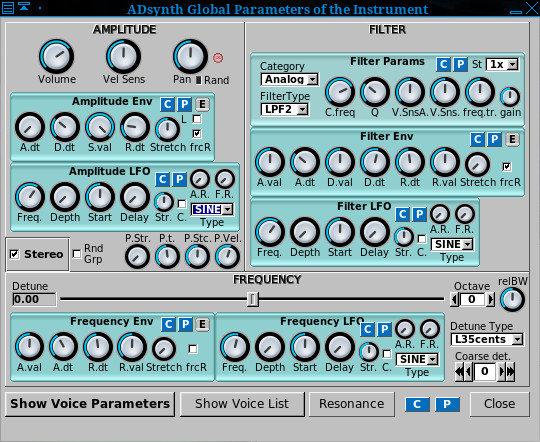
\includegraphics[scale=1.0]{bottom-panel/instrument-edit/ADD/ADDsynth-edit.jpg}
   \caption{ADDsynth Edit/Global Dialog}
   \label{fig:addsynth_edit_dialog}
\end{figure}

   The major sections of this dialog are listed:

   \begin{enumber}
      \item \textbf{AMPLITIUDE} (section)
      \item \textbf{FILTER} (section)
      \item \textbf{FREQUENCY} (section)
      \item \textbf{Show Voice Parameters} (section)
      \item \textbf{Show Voice List} (section)
      \item \textbf{Resonance} (section)
      \item \textbf{C}
      \item \textbf{P}
      \item \textbf{Close}
   \end{enumber}

   This complex dialog is best described section by section.
   Many of the sub-sections are stock sub-panels described elsewhere
   in this document.

\subsection{ADDsynth / AMPLITUDE}
\label{subsec:addsynth_amplitude}

   \begin{enumber}
      \item \textbf{Volume}
      \item \textbf{Vel Sens}
      \item \textbf{Pan}
      \item \textbf{Rand}
      \item \textbf{Reset (panning)} (red button)
      \item \textbf{Amplitude Env}
         The Amplitude Env panel is described in detail in
         \sectionref{subsubsec:amplitude_envelope_subpanel}.
%        section~\ref{subsubsec:amplitude_envelope_subpanel} on
%        page~\pageref{subsubsec:amplitude_envelope_subpanel}.
      \item \textbf{Amplitude LFO}
         The Amplitude LFO panel is described in detail in
         \sectionref{subsubsec:lfo_user_interface_panels}.
%        section~\ref{subsubsec:lfo_user_interface_panels} on
%        page~\pageref{subsubsec:lfo_user_interface_panels}.
      \item \textbf{Stereo}
      \item \textbf{Rnd Grp}
      \item \textbf{P.Str.}
      \item \textbf{P.t}
      \item \textbf{P.Stc.}
      \item \textbf{P.Vel.}
   \end{enumber}

   Note the two sub-panels, mentioned above, that are described elsewhere.
   They will not be mentioned below.

   \setcounter{ItemCounter}{0}      % Reset the ItemCounter for this list.

   \itempar{Volume}{addsynth!volume}
   ADDsynth Volume.

   Values: \texttt{1 to 127, 64*}

   Sets the overall/relative volume of the instrument.

   \itempar{Vel Sens}{addsynth!vel sens}
   ADDsynth Velocity Sensing function.
   Turn the knob rightmost/maximum to disable this function.

   Values: \texttt{1 to 127, 64*}

   Velocity sensing is simply an exponental transformation from the note’s
   velocity to some parameter change.
   Observe \figureref{fig:velocity_sensing_function}.
   It shows how the velocity sensing controls affects the translation of a
   parameter over the whole range of possible note velocities.

\begin{figure}[H]
   \centering 
   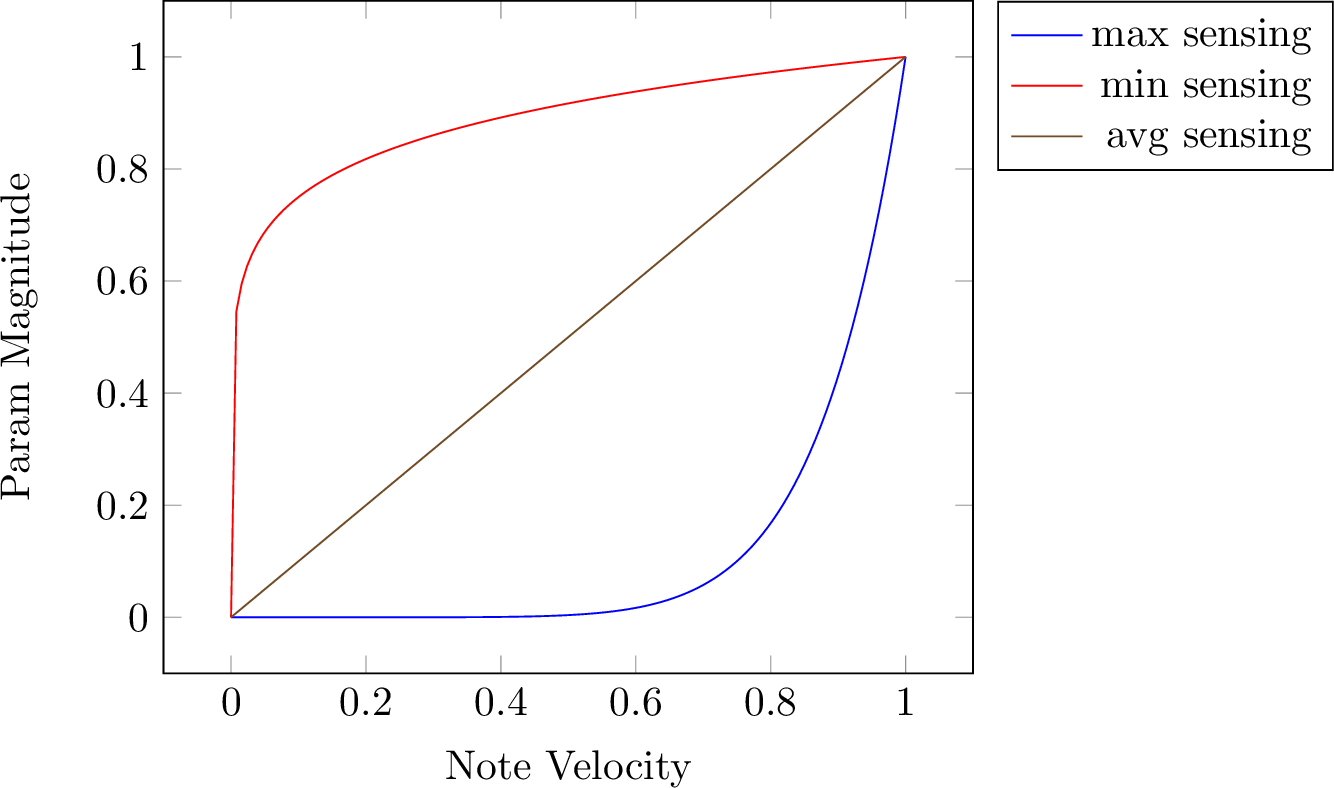
\includegraphics[scale=0.25]{zyn/velocity_sensing_function_velf.png}
   \caption{Velocity Sensing Function}
   \label{fig:velocity_sensing_function}
\end{figure}

   \itempar{Pan}{addsynth!pan}
   ADDsynth Global Panning.

   Values: \texttt{0, 1 to 127, 64*}

   Dialing the knob to leftmost or zero gives random panning.

   \itempar{Rand}{addsynth!random pan}
   ADDsynth Random Panning Indicator.
   A red fill-in color provides an indicator for the activation of random
   panning in this control.

   \itempar{Reset (panning)}{addsynth!reset pan}
   ADDsynth Reset Panning (red button).
   Clicking this red button changes the panning value to 64 (centered).

   Next, we skip the \textbf{Amplitude Env} and \textbf{Amplitude LFO}
   panels, which are described elsewhere, as noted above.

   \itempar{Stereo}{addsynth!Stereo}
   ADDsynth Stereo.

   Values: \texttt{Off, On*}

   Stereo can be enabled.
   When disabled, all the voices will also have panning disabled.

   \itempar{Rnd Grp}{addsynth!group}
   ADDsynth Random Group.

   Values: \texttt{Off*, On}

   How the harmonic amplitude is applied to voices that use the same
   oscillator.

   TODO:  Get a more detailed explanation of what this setting means.

   \itempar{P.Str.}{addsynth!punch strength}
   ADDsynth Punch Strength.

   Values: \texttt{0* to 127}

   The punch strength of a note in ADDsynth is a constant amplification to
   the output at the start of the note, with its length determined by the
   punch time and stretch and the amplitude being determined by the punch
   strength and velocity sensing. The \textbf{relBW}
   control in the frequency panel is
   effectively a multiplier for detuning all voices within an ADnote.

   \itempar{P.t}{addsynth!punch time}
   ADDsynth Punch Time (duration).

   Values: \texttt{0 to 127, 64*}

   Sets the punch effect duration (from 0.1 ms to 100 ms on an A note, 440Hz).

   \itempar{P.Stc.}{addsynth!punch stretch}
   ADDsynth Punch Stretch.

   Values: \texttt{0 to 127, 64*}

   Sets the punch effect stretch according to frequency. On lower-frequency
   notes, punch stretch makes the punch effect last longer. 

   \itempar{P.Vel.}{addsynth!punch vel sens}
   ADDsynth Punch Velocity Sensing.

   Values: \texttt{0 to 127, 72*}

   The higher this value, the higher the effect of velocity on the punch of
   the note.

\subsection{ADDsynth / FILTER}
\label{subsec:addsynth_filter}

   The ADDsynth FILTER block consists solely of sub-panels
   described in detail in the sections noted below.  The
   sub-panels of the FILTER section are:

   \begin{enumber}
      \item \textbf{Filter Params}
      \item \textbf{Filter Env}
      \item \textbf{Filter LFO}
   \end{enumber}

   \setcounter{ItemCounter}{0}      % Reset the ItemCounter for this list.

   \itempar{Filter Params}{addsynth!filter params}
   ADDsynth Filter Parameters.
   The Filter Params panel is described in detail in
   \sectionref{subsubsec:filter_parameters_user_interface}.

   \itempar{Filter Env}{addsynth!filter env}
   ADDsynth Filter Envelope.
   The Filter Env panel is described in detail in
   \sectionref{subsubsec:envelope_settings_for_filter}.

   \itempar{Filter LFO}{addsynth!filter lfo}
   The Filter LFO panel is described in detail in
   \sectionref{subsubsec:lfo_user_interface_panels}.

\subsection{ADDsynth / FREQUENCY}
\label{subsec:addsynth_frequency}

   \begin{enumber}
      \item \textbf{Detune}
      \item \textbf{FREQUENCY slider}
      \item \textbf{Octave}
      \item \textbf{RelBW}
      \item \textbf{Frequency Env}.
         A stock sub-panel described in
         \sectionref{subsubsec:envelope_settings_for_frequency}.
      \item \textbf{Frequency LFO}
         A stock sub-panel described in
         \sectionref{subsubsec:frequency_lfo_sub_panel}.
      \item \textbf{Detune Type}
      \item \textbf{Coarse det.}
   \end{enumber}

   \setcounter{ItemCounter}{0}      % Reset the ItemCounter for this list.

   \itempar{Detune}{addsynth!detune value}
   ADDsynth Detune Value.
   This display box shows the value of the detune as selected by the
   frequency slider described below.

\begin{figure}[H]
   \centering 
   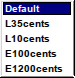
\includegraphics[scale=1.0]{bottom-panel/instrument-edit/ADD/frequency-detune-type.jpg}
   \caption{ADDsynth Frequency Detune Type}
   \label{fig:addsynth_freq_detune_type}
\end{figure}

   Values: \texttt{-35.00 to 35.00, 0*}

   \itempar{FREQUENCY slider}{addsynth!freq slider}
   ADDsynth Fine Detune (cents), a slider control.

   Values: \texttt{-35.00 to 35.00}

   While the detune type dropdown and the octave selection provide a coarse
   selection of detune, the slider allows for a finer selection of detune.

   \itempar{Octave}{addsynth!octave}
   ADDSynth Octave.

   Values: \texttt{-8 to 7, 0*}

   The octave setting changes the frequency by octaves.

   \itempar{RelBW}{addsynth!relative bw}
   ADDSynth Relative Bandwidth.

   Values: \texttt{0 to 127, 64*}

   Bandwidth: how the relative fine detune of the voice is changed.

   \itempar{Frequency Env}{addsynth!frequency env}
   ADDsynth Frequency Envelope.
   The Frequency Env panel is described in detail in
   \sectionref{subsubsec:envelope_settings_for_frequency}.

   \itempar{Frequency LFO}{addsynth!frequency lfo}
   The Frequency LFO panel is described in detail in
   \sectionref{subsubsec:lfo_user_interface_panels}

   \itempar{Detune Type}{addsynth!detune type}
   Frequency Detune Type.

   Values: \texttt{L35cents, L10cents, E100cents, E1200cents}

   This setting provides a coarse detuning.
   We would welcome an explanation of exactly is meant by the numbers and
   the "E" versus "L" designation.

   \itempar{Coarse det.}{addsynth!coarse detune}
   Coarse Detune, "C.detune".

   Values: \texttt{-64 to 63, 0*}

   The one-arrow buttons change the value by one.
   The two-arrow buttons change the value by ten.

   Again, we need a way to explain the interactions of the slider, the
   octave setting, the detune type, and the coarse detune settings.

   \itempar{Show Voice Parameters}{addsynth!voice parameters}
   ADDsynth Show Voice Parameters.
   This button brings up the following "voice parameters" dialog.
   Again, this dialog is built from some stock sections and stock
   sub-panels, plus additional elements.

\subsection{ADDsynth / Voice Parameters}
\label{subsec:addsynth_voice_parameters}

   Each \textsl{Yoshimi} ADDsynth instrument consists of up to 8 voices.
   This dialog provides a way to define each of the 8 voices in great
   detail.

\begin{figure}[H]
   \centering 
   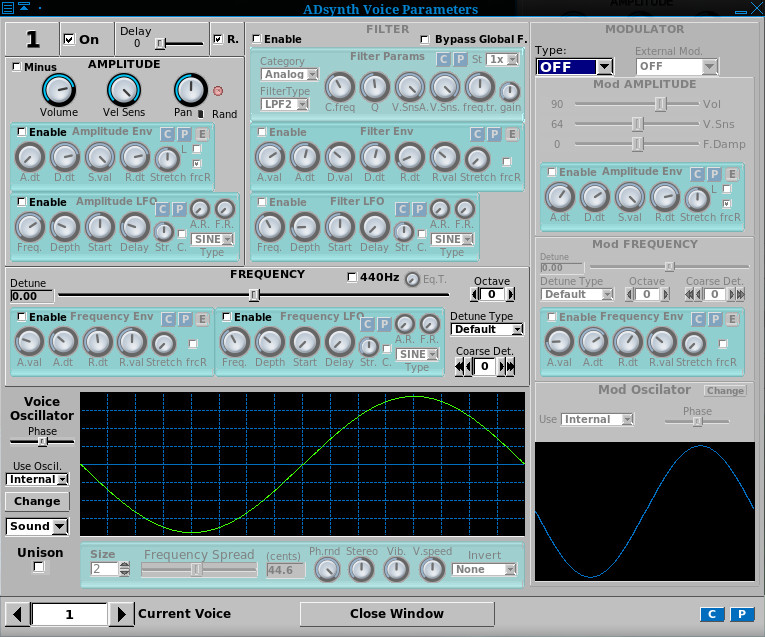
\includegraphics[scale=0.75]{bottom-panel/instrument-edit/ADD/ADDsynth-voice-parameters.jpg}
   \caption{ADDsynth Voice Parameters Dialog}
   \label{fig:addsynth_voice_parameters_dialog}
\end{figure}

   This dialog consists of a few extra settings, plus a number of
   stock dialog sections.

   \begin{enumber}
      \item \textbf{Voice Number}
      \item \textbf{On}
      \item \textbf{Delay}
      \item \textbf{R.}
      \item \textbf{AMPLITUDE} (see section below)
      \item \textbf{FILTER} (see section below)
      \item \textbf{MODULATOR} (see section below)
      \item \textbf{FREQUENCY} (see section below)
   \end{enumber}

   \setcounter{ItemCounter}{0}      % Reset the ItemCounter for this list.

   \itempar{Voice Number}{voice!number}
   ADDsynth Voice Number.

   Values: \texttt{1* to 8}

   This display element shows the voice number represented by the settings
   in this dialog.  Each \textsl{Yoshimi} part/instrument can consist of up
   to eight voices.

   The voice being worked on can be selected using the
   \textbf{Current Voice} selector.

   \itempar{On}{voice!on/off}
   ADDsynth Voice On/Off.

   Values: \texttt{Off, On}

   Enables this voice in the part/instrument.

   \itempar{Delay}{voice!delay}
   ADDsynth Voice Delay.

   Values: \texttt{0* to 127}

   TODO: We still need to determine what the units of the delay are.

   \textbf{Bug:}
   \index{bugs!ADDsynth voice delay tooltip}
   The tooltip for this setting says "Volume".

   \itempar{R.}{voice!resonance}
   ADDsynth Voice Resonance On/Off.

   Values: \texttt{Off, On*}

   TODO: It is not clear what effect this has, as there seems to be no way
   to edit "resonance" in this dialog.

   The rest of the GUI elements
   (AMPLITUDE, FILTER, MODULATOR, FREQUENCY, and Voice Oscillator)
   are more detailed, and discussed in the sections that follow.

\subsubsection{ADDsynth / Voice Parameters / AMPLITUDE}
\label{subsubsec:addsynth_voice_parameters_amplitude}

   This section of the voice parameters dialog also includes a couple of
   stock sub-panels that have an additional "Enable" control.

   \begin{enumber}
      \item \textbf{Minus}
      \item \textbf{Volume}
      \item \textbf{Vel Sens}
      \item \textbf{Pan}
      \item \textbf{Pan randomness indicator}
      \item \textbf{Pan reset} (red button)
      \item \textbf{Amplitude Env, Stock + Enable}
      \item \textbf{Amplitude LFO, Stock + Enable}
   \end{enumber}

   \setcounter{ItemCounter}{0}      % Reset the ItemCounter for this list.

   \itempar{Minus}{voice par amp!invert vol control}
   ADDsynth Amplitude Minus.

   Values: \texttt{Off*, On}

   This setting enables the inversion of the volume control action.
   It enables negative values for the volume control of the voice.

   \itempar{Volume}{voice par amp!volume}
   ADDsynth Voice Volume.

   Values: \texttt{0 to 127, 90?}

   Sets the (relative) volume of this voice in the part/instrument.

   \itempar{Vel Sens}{voice par amp!vel sens}
   ADDsynth Voice velocity-sensing function; setting to rightmost/max
   disables this function.

   Values: \texttt{0 to 127*}

   \itempar{Pan}{voice par amp!pan}
   ADDsynth Voice panning; setting to leftmost/0 gives random panning.

   Values: \texttt{0 to 127, 64*}

   \itempar{Pan randomness indicator}{voice par amp!random pan}
   ADDsynth Voice random panning On/Off.
   Fills in red to indicate that random panning is in force.

   \itempar{Pan reset (red button)}{voice par amp!center pan}
   ADDsynth Center Panning.

   Clicking this small red button resets the panning to center.

   \itempar{Amplitude Env, Stock + Enable}{voice par amp!amp env}
   ADDsynth Amplitude Envelope Sub-panel.
   See \sectionref{subsubsec:amplitude_envelope_subpanel}.
   Additionally, the \textbf{Enable} checkbox allows the enabling of this
   component.

   \itempar{Amplitude LFO, Stock + Enable}{voice par amp!amp lfo}
   ADDsynth Amplitude LFO Sub-panel.
   See \sectionref{subsubsec:lfo_user_interface_panels}.
   Additionally, the \textbf{Enable} checkbox allows the enabling of this
   component.

\subsubsection{ADDsynth / Voice Parameters / FILTER}
\label{subsubsec:addsynth_voice_parameters_filter}

   This section of the voice parameters dialog also includes a couple of
   stock sub-panels that have an additional "Enable" control.

   \begin{enumber}
      \item \textbf{Enable}
      \item \textbf{Bypass Global F.}
      \item \textbf{Filter Params, Stock}
      \item \textbf{Filter Env, Stock + Enable}
      \item \textbf{Filter LFO, Stock + Enable}
   \end{enumber}

   \setcounter{ItemCounter}{0}      % Reset the ItemCounter for this list.

   \itempar{Enable}{voice par filter!enable}
   ADDsynth Voice Enable Filter.

   Values: \texttt{Off*, On}

   This value enables the whole FILTER dialog section.

   \itempar{Bypass Global F.}{voice par filter!bypass}
   ADDsynth Voice Bypass Global Filter.

   Values: \texttt{Off*, On}

   The voice signal bypasses the global filter.
   TODO:  Make sure there is a discussion of the global filter.

   \itempar{Filter Params, Stock}{voice par filter!parameters}
   See \sectionref{subsubsec:filter_parameters_user_interface}.

   \itempar{Filter Env, Stock + Enable}{voice par filter!env}
   See \sectionref{subsubsec:envelope_settings_for_filter}.

   \itempar{Filter LFO, Stock + Enable}{voice par filter!lfo}
   See \sectionref{subsubsec:filter_lfo_sub_panel}.

\subsubsection{ADDsynth / Voice Parameters / MODULATOR}
\label{subsubsec:addsynth_voice_parameters_modulator}

   \begin{enumber}
      \item \textbf{Type:}
      \item \textbf{External Mod.}
      \item \textbf{Mod AMPLITUDE}
      \item \textbf{Mod FREQUENCY}
      \item \textbf{Mod Oscillator}
   \end{enumber}

   \setcounter{ItemCounter}{0}      % Reset the ItemCounter for this list.

   \itempar{Type:}{modulator!type}
   ADDsynth Modulator Type.

   Values: \texttt{OFF(, MORPH, RING, PM, FM, PITCH}

\begin{figure}[H]
   \centering 
   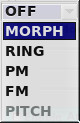
\includegraphics[scale=1.0]{bottom-panel/instrument-edit/ADD/modulator-type.jpg}
   \caption{Voice Modulator Type}
   \label{fig:voice_modulator_type}
\end{figure}

   \begin{enumber}
      \item \textbf{OFF}.
      This setting turns off the modulator.
      \item \textbf{MORPH}
      The morph modulator works by combining the output of two oscillators
      into one, with the amplitude envelope translating between one waveform
      and the other.
      \item \textbf{RING}
      The ring modulator is useful for making bell-like sounds and some weird
      effects.  The ring modulator works by multiplying two waveforms
      together, producing a signal that is the sum and difference of the
      frequencies present in the waveforms.  The ins-and-outs of the ring
      modulator are explained in detail in
      paragraph~\ref{paragraph:tip_using_the_ring_modulator}.
      \item \textbf{PM}
      The PM (pulse modulation) modulator works by using a modulator
      envelope to change the pulse width of a pulse waveform.
      Generally, set \textbf{F.Damp} to zero, so that the modulation amount
      doesn't depend on the note number.
      \item \textbf{FM}
      The (frequency modulation) morph modulator works by modulator the
      frequency.  Examples can be heard in the "Ethereal" and "Steel Wire"
      instruments.
      \item \textbf{PITCH}
      The pitch modulator works by...
      we're not sure... is this pitch shifting?
   \end{enumber}

   \itempar{External Mod.}{modulator!external}
   External Oscillator.
   External Modulator.

   Values: \texttt{OFF*, Other voice numbers?}

   TODO: Make sure this description is right!

   \textbf{External Oscillator}.
   This feature allows one of the voices (of the up to 8 allowed in a single
   ADDsynth instrument) to be used as a modulator or external oscillator for
   another voice in the instrument.
   This option specifies to use the oscillator of another voice, or
   -1 for the \textsl{internal} oscillator.

   The parameters must be lower than the voice index, One cannot use the
   oscillator from a voice with a bigger index (one can't use the oscillator
   of voice 8 for voice 4). This is very useful because, if one uses
   many voices with the same oscillator settings, one can use only one
   oscillator and select other voices to use this; if one changes a parameter
   of the oscillator, all voices using this oscillator will be affected.

   \textbf{External Modulator}.
   Use another voice as a modulator instead of the modulator of the internal
   voice. One can make a modulation "stack". The modulator of the voice is
   disabled. 

   External. Uses the oscillator as the modulator of another voice. It
   behaves like "Ext. Oscil" except that it works on the
   \textsl{modulator}. Please
   notice the difference between this parameter and \textbf{Ext. Mod}. 

   See below.

   \itempar{Mod AMPLITUDE}{modulator!amplitude}
   Modulator Amplitude.

   \begin{enumber}
      \item \textbf{Vol}
         Volume.
         Values: \texttt{0 to 127, 90*}
      \item \textbf{V.Sns}
         Velocity Sensing Function - rightmost/max to disable.
         Values: \texttt{0 to 127, 64*}
      \item \textbf{F.Damp}
         Modulator Damp at higher frequency.
         How the modulator intensity is lowered according to lower/higher
         note frequencies. 
         Values: \texttt{0 to 127, 90*}
      \item \textbf{Amplitude Env, Stock + Enable}
         See section....
   \end{enumber}

   \itempar{Mod FREQUENCY}{modulator!frequency}
   Modulator Frequency.

   \begin{enumber}
      \item \textbf{Detune slider}
         Fine Detune (cents).
         Values: \texttt{-35.00 to 35.00, 0*}
      \item \textbf{Detune Type}
         Fine Detune (cents).
         Values: \texttt{L35cents, L10cents, E100cents, E1200cents}
         See figure~\ref{fig:addsynth_freq_detune_type} on
         page~\pageref{fig:addsynth_freq_detune_type}.
      \item \textbf{Octave}
         Octave.
         Values: \texttt{-8 to 7, 0*}
      \item \textbf{Coarse Det.}
         Coarse Detune.
         Values: \texttt{-64 to 63, 0*}
      \item \textbf{Filter Env, Stock + Enable}
         See section...
   \end{enumber}

   \itempar{Mod Oscillator}{modulator!oscillator}
   Modulator Oscillator.

   \textbf{Bug:}
   \index{bugs!mod oscillator name mispelled}
   The word "oscillator" is mispelled in the application.

   \begin{enumber}
      \item \textbf{Change}
         ADDsynth Oscillator Editor.
      \item \textbf{Use}
         Oscillator to Use.
         See the paragraph below.
         Values: \texttt{Internal*, Other oscillators?}
      \item \textbf{Phase}
         Oscillator Phase.
         Values: \texttt{0 to 360 (0 to 2PI)}
      \item \textbf{Waveform graph}
         Waveform graph.
   \end{enumber}

   As far as we can tell, one has the choice between Internal, which in this
   case means a completely independent modulator oscillator per voice (extra
   change button), or External, which refers to the Modulation
   oscillators one has already defined for the voices with a lower index.
   This means one can make one modulation oscilator for voice 1, and reuse it
   in voice 2 and 3.  This is the same system as is used for the normal
   oscillators.

\paragraph{Tip: Using the Ring Modulator}
\label{paragraph:tip_using_the_ring_modulator}
\index{tip!ring modulator}
\index{tip!internal modulator}

   This section is derived from on the short text files in the
   \textsl{Yoshimi} source-code bundle.  It notes that "Some people have
   been confused about how to use an 'external' Mod Oscillator", and
   provides usage notes that we will elaborate on here.  Here is the way to
   use it:

   \begin{enumber}
      \item Open the ADDsynth editing window.  Then open
         \textbf{Show Voice Parameters}.
      \item For \textbf{Type}, select the \textbf{RING} value.  This
      selection will activate the \textbf{Mod Oscillator}.
      \item In the \textbf{Mod Oscillator}, click on \textbf{Change} to open
      the \textbf{ADDsynth Oscillator Editor}.
      \item Set the wave-shape to \textbf{Triangle}.
      \item Switch to voice number 2 and enable it.
      \item Again, for \textbf{Type}, select the \textbf{RING} value.
      However, feel free to select one of the other modulators, if one
      wishes.
      \item One can now use \textbf{Internal} for voice 2, or select
      \textbf{ext.m} 1, to use the first voice as in internal modulator.
      \item Change the internal voice to, for example, \textbf{Square}.
      \item Do the same setup for voice 3.
      One will find that one can use its \textbf{Internal} or
      either of the two previous ones.
   \end{enumber}

   Now the joker in the pack is that one can disable both the previous
   voices but \textsl{still} use their Mod Oscillators.

   What is going on here?  Need to explain better!!!!!

   In a newsgroup (\cite{ringmodulator}, the following note is found.

   \begin{quotation}
      Say I want the A tone ring-modulated by 880Hz. A is 440 Hz, the ring
      modulation setting lets me choose the modulation frequency relative
      to the frequency of the tone. So I choose octave 1 and let the
      detune at zero. If I move the detune, it'll shift the modulation
      frequency a bit, which will make a disharmonic effect.

      Wet/dry setting is controlled by volume in "modulation amplitude".
      The modulation frequency can further be multiplied or several
      modulations can be simulated by changing the oscillator waveform.

      One huge letdown is that it is only available for Adsynth. PadSynth
      does not seem to have ring modulation option, so the coolest sounds
      stay out of question for massive lead tones. :-(
   \end{quotation}

\subsubsection{ADDsynth / Voice Parameters / FREQUENCY}
\label{subsubsec:addsynth_voice_parameters_frequency}

   % Similar to the ADDsynth Edit's FREQUENCY section.

   Frequency section, almost a stock part.

   \begin{enumber}
      \item \textbf{Detune}
      \item \textbf{FREQUENCY slider}
      \item \textbf{440 Hz}         % addition to stock
      \item \textbf{Eq.T.}          % addition to stock
      \item \textbf{Octave}
      \item \textbf{Detune Type}
      \item \textbf{Coarse det.}
      \item \textbf{Frequency Env, Stock + Enable}
      \item \textbf{Frequency LFO, Stock + Enable}
      \item \textbf{Voice Oscillator}
   \end{enumber}

   \setcounter{ItemCounter}{0}      % Reset the ItemCounter for this list.

   \itempar{Detune}{voice parameters!detune}
   Voice Parameters Detune.

   Values: \texttt{-35.00 to 35.00, 0*}

   \itempar{FREQUENCY slider}{voice parameters!freq slider}
   Frequency Slider.

   \itempar{440 Hz}{voice parameters!440 hz}
   440Hz.

   Values: \texttt{Off*, On}

   Fix the base frequency to 440Hz.
   One can adjust this with the detune settings.

   TODO: Occurs in which panels?

   \itempar{Eq.T.}{voice parameters!eq type}
   Equalization type?  Additional.

   Values: \texttt{0 to 127?}

   Occurs in which panels?

   \itempar{Octave}{voice parameters!octave}
   Voice Paramaters Octave.

   Values: \texttt{-8 to 7, 0*}

   \itempar{RelBW}{voice parameters!relbw}
   Relative bandwidth.

   \itempar{Detune Type}{voice parameters!fine detune}
   Fine Detune (cents). ?????

   Values: \texttt{L35cents, L10cents, E100cents, E1200cents}

\begin{figure}[H]
   \centering 
   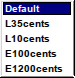
\includegraphics[scale=1.0]{bottom-panel/instrument-edit/ADD/frequency-detune-type.jpg}
   \caption{Frequency Detune TYpe}
   \label{fig:frequency_detune_tYpe}
\end{figure}

   \itempar{Coarse det.}{voice parameters!coarse detune}
   Coarse Detune.

   Values: \texttt{-64 to 63, 0*}

   \itempar{Frequency Env, Stock + Enable}{voice parameters!freq env}
   Frequency Envelope.

   \itempar{Frequency LFO, Stock + Enable}{voice parameters!freq lfo}
   Frequency LFO.

   \itempar{Voice Oscillator}{voice parameters!oscillator}
   Voice Parameters Oscillator.
   See next section.

\subsubsection{ADDsynth / Voice Parameters / Voice Oscillator}
\label{subsubsec:addsynth_voice_parameters_oscillator}

   \begin{enumber}
      \item \textbf{Phase}
      \item \textbf{Use}
      \item \textbf{Waveform graph}
      \item \textbf{Change}
      \item \textbf{Sound}
      \item \textbf{Unison}
      \item \textbf{Current Voice}
      \item \textbf{C}
      \item \textbf{P}
      \item \textbf{Close Window}
   \end{enumber}

   \setcounter{ItemCounter}{0}      % Reset the ItemCounter for this list.

   \itempar{Phase}{voice oscillator!phase}
   Voice Oscillator Phase.

   Values: \texttt{0 to 360 (0 to 2*pi)}

   \itempar{Use Oscil.}{voice oscillator!use}
   Use Oscillator.

   Values: \texttt{Internal*, Other oscillators?}

   \itempar{Waveform graph}{voice oscillator!waveform}
   Waveform Graph.

   \itempar{Change}{voice oscillator!Change}
   Voice Oscillator Change,
   ADDsynth Oscillator Editor.

\begin{figure}[H]
   \centering 
   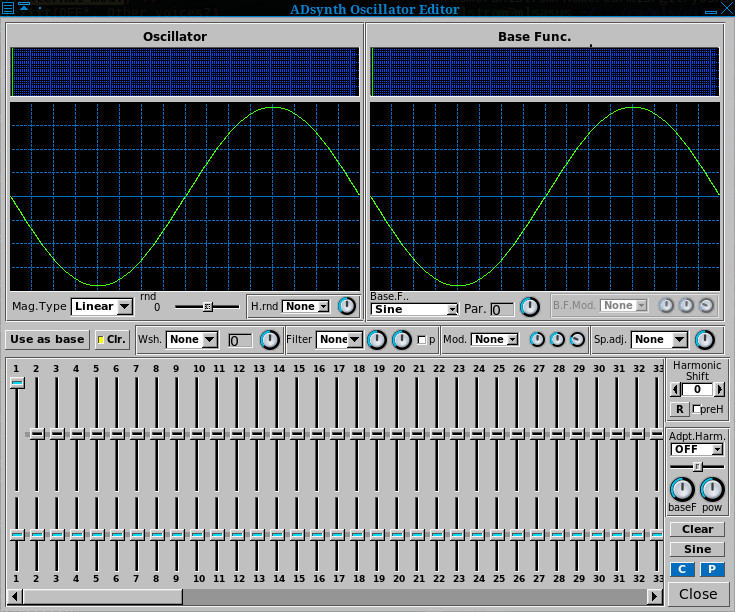
\includegraphics[scale=0.75]{bottom-panel/instrument-edit/ADD/ADDsynth-oscillator-editor.jpg}
   \caption{ADDsynth Oscillator Editor}
   \label{fig:addsynth_oscillator_editor}
\end{figure}

   This item is identical to the PADsynth harmonic editor described in
   section~\ref{subsubsec:padsynth_harmonic_structure_change} on
   page~\pageref{subsubsec:padsynth_harmonic_structure_change}.

   \itempar{Sound}{voice oscillator!sound}
   Oscillator Type (sound/noise).
   Sound/Noise choice.
   Select the mode of the oscillator (sound versus white noise).

\begin{figure}[H]
   \centering 
   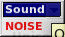
\includegraphics[scale=1.0]{bottom-panel/instrument-edit/ADD/voice-oscillator-sound-dropdown.jpg}
   \caption{Voice Oscillator Choices}
   \label{fig:voice_oscillator_choices}
\end{figure}

   Values: \texttt{Internal*, Other oscillators?}

   \itempar{Unison}{voice oscillator!Unison}
   Unison is useful in creating the chorus like sound of many simultaneous
   oscillators.

   Values: \texttt{Off*, On}

   Enabling this item causes the following items to become enabled.

      \begin{enumber}
         \item \textbf{Size}
         Number of unison sub-voices.
         Values: \texttt{2* to 50}
         \item \textbf{Frequency Spread}
         Frequency spread of the unison (cents).
         Values: \texttt{0 to 200, 44.6*}
         \item \textbf{Ph.rnd}
         Phase randomness.
         Values: \texttt{0 to 127*}
         \item \textbf{Stereo}
         Stereo Spread.
         Values: \texttt{0 to 127, 64*}
         \item \textbf{Vibrato}
         Vibrato.
         Values: \texttt{0 to 127, 64*}
         \item \textbf{V.speed}
         Vibrato Average Speed.
         Values: \texttt{0 to 127, 64*}
         \item \textbf{Invert}
         Phase Invert.
         Values: \texttt{None*, Random, 50\%, 33\%, 25\%, 20\%}
      \end{enumber}

\begin{figure}[H]
   \centering 
   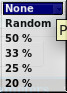
\includegraphics[scale=1.0]{bottom-panel/instrument-edit/ADD/voice-oscillator-phase-invert-dropdown.jpg}
   \caption{Phase Invert Dropdown}
   \label{fig:phase_invert_dropdown}
\end{figure}

   \itempar{Current Voice}{voice oscillator!current voice}
   Current Voice.

   Values: \texttt{1* to 8}

   \itempar{C}{voice oscillator!copy}
   Copy D note parameters.

   \itempar{P}{voice oscillator!paste}
   Paste D note parameters.

   \itempar{Close Window}{voice oscillator!close}
   Close.

   % HERE
   % HERE
   % HERE

\subsection{ADDsynth / Voice List}
\label{subsec:addsynth_voice_list}

   ADsynth Voices List (Voices 1 to 8).

\begin{figure}[H]
   \centering 
   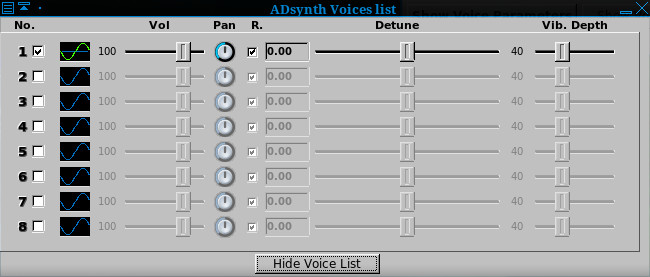
\includegraphics[scale=1.0]{bottom-panel/instrument-edit/ADD/ADDsynth-voices-list.jpg}
   \caption{ADDsynth Voices List}
   \label{fig:addsynth_voices_list}
\end{figure}

   \begin{enumber}
      \item \textbf{No. (1 to 8)}
      \item \textbf{Vol}
      \item \textbf{Pan}
      \item \textbf{R.}
      \item \textbf{Detune}
      \item \textbf{Vib. Depth}
      \item \textbf{Hide Voice List}
   \end{enumber}

   \setcounter{ItemCounter}{0}      % Reset the ItemCounter for this list.

   \itempar{No. (1 to 8)}{voice list!number}
   Voice List Number.

   Values: \texttt{Off, On} ???

   \itempar{Vol}{voice list!volume}
   Voice Volume.

   Values: \texttt{0 to 127, 100*}

   \itempar{Pan}{voice list!panning}
   Voice Panning (0/leftmost is Random).

   Values: \texttt{0 to 127, 64*}

   \itempar{R.}{voice list!resonance}
   Resonance On/Off.
   Enable/disable the resonance effect of a voice.

   Values: \texttt{Off, On*}

   \itempar{Detune}{voice list!detune}
   Fine Detune (cents).

   Values: \texttt{-35 to 35, 0*}

   \itempar{Vib. Depth}{voice list!vibrato depth}
   Frequency LFO Amount/Depth.
   This setting can be very useful because, with the detune settings, one can
   create very good sounding instruments. 

   Values: \texttt{0 to 127, 40*}

   \itempar{Hide Voice List}{voice list!hide}
   Hide Voice List.  A Close button, really.

\subsection{ADDsynth / Resonance}
\label{subsec:addsynth_resonance}

   The resonance effect acts as a "resonance box" or a filter with arbitrary
   frequency response. This produces very realistic sounds. 
   The cursor location is shown below the graph (the frequency - kHz and
   amplitude - dB). 

\begin{figure}[H]
   \centering 
   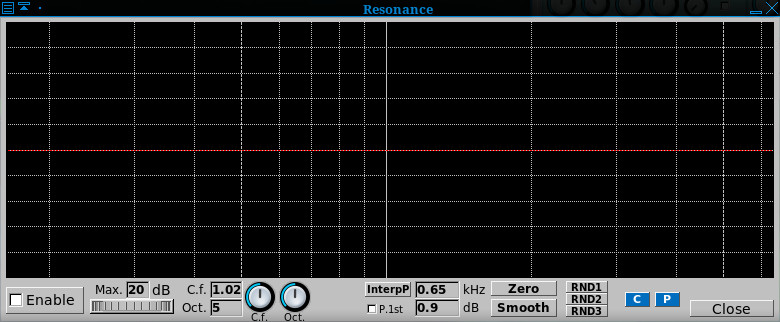
\includegraphics[scale=0.75]{bottom-panel/instrument-edit/ADD/ADDsynth-resonance.jpg}
   \caption{ADDsynth Resonance}
   \label{fig:addsynth_resonance}
\end{figure}

   \begin{enumber}
      \item \textbf{Graph Window}
      \item \textbf{Enable}
      \item \textbf{Max dB (wheel)}
      \item \textbf{C.f. (knob)}
      \item \textbf{Oct.}
      \item \textbf{P.1st}
      \item \textbf{InterpP}
      \item \textbf{KHz}
      \item \textbf{dB}
      \item \textbf{Zero}
      \item \textbf{Smooth}
      \item \textbf{RND1}
      \item \textbf{RND2}
      \item \textbf{RND3}
      \item \textbf{C}
      \item \textbf{P}
      \item \textbf{Close}
   \end{enumber}

   \setcounter{ItemCounter}{0}      % Reset the ItemCounter for this list.

   \itempar{Graph Window}{resonance!graph}
   Resonance Graph Window.
   Lets one draw in "freehand" mode.

   \itempar{Enable}{resonance!Enable}
   Resonance Enable.
   Turn the Resonance effect on.

   Values: \texttt{Off*, On}

   \itempar{Max dB (wheel)}{resonance!max db}
   The Maximum Amplitude (dB) wheel.
   Sets the amount of resonance: lower values have little effect. Use the
   roller below to set it. 

   Values: \texttt{1 to 90, 20*}

   \itempar{C.f. (knob)}{resonance!cf}
   Center Frequency (kHz).
   Sets the center frequency of the graph.

   Values: \texttt{0 to 127, 64*} for \texttt{0.10 to 10.0, 1.0*}

   \itempar{Oct.}{resonance!octaves}
   Number of Octaves.
   Sets the number of octaves the graph represents.

   Values: \texttt{0 to 127, 64*} for \texttt{0 to 10, 5*}

   \itempar{P.1st}{resonance!first harmonic}
   Protect the fundamental Frequency.
   Do not damp the first harmonic.

   Values: \texttt{Off, On}

   \itempar{InterpP}{resonance!interpolate}
   Interpolate the peaks.
   This one is a weird one where mouse movement affects it,
   but also affects the next field as well.  Oh, kHz and dB.

   This setting allows one to make resonance functions very easily. First,
   clear the graph using the "Zero" button. Click the left button on a
   position on the graph. Click the "InterpP" button. It will interpolate
   automatically between the positions pointed to (or drew).  Also one can
   clear a part of the graph by dragging with the right mouse button. In
   fact, the "interpP" button interpolates between non-zero values.  If one
   presses the "InterpP" with the right mouse button, the interpolation will
   be linear, and if one uses the left button, the interpolation will be
   smooth. 

   \itempar{KHz}{resonance!khz}
   The current frequency on graph.

   \itempar{dB}{resonance!db}
   The current level on graph window.

   Values: \texttt{-90 to +90}

   \itempar{Zero}{resonance!clear}
   Clear the resonance function.
   Zero. Clear the graph.

   Amplification - how the output signal is amplified (WHERE?)

   \itempar{Smooth}{resonance!smooth}
   Smooth the resonance function.
   Smooth the graph.

   \itempar{RND1}{resonance!randomize}
   Randomize the resonance function, 1.
   RND1, RND2, RND3 are used to create random resonance functions.

   \itempar{RND2}{resonance!randomize}
   Randomize the resonance function, 2.

   \itempar{RND3}{resonance!randomize}
   Randomize the resonance function, 3.

   \itempar{C}{resonance!copy}
   Copy Dialog.

   \itempar{P}{resonance!paste}
   Paste Dialog.

   \itempar{Close}{resonance!close}
   Close.

%-------------------------------------------------------------------------------
% vim: ts=3 sw=3 et ft=tex
%-------------------------------------------------------------------------------
